\chapter{System Architecture}
\thispagestyle{plain}
\section*{Introduction}
\addcontentsline{toc}{section}{Introduction}
This chapter examines the delivered architecture as a running system rather than as an idealized diagram. It explains the service topology, the division of responsibilities, the trust boundaries, the data model, the frontend proxy pattern, the authentication and secret-management flows, and the request paths that connect them.

\section{Why This Architecture and Not Another}
Architectural discussion is often weakened by starting from the chosen design and treating it as self-justifying. A stronger approach is to articulate the competing architectural options and the reasons they were not selected.

For this project, there were at least three plausible structural choices. A classic monolith would have simplified deployment and debugging, but it would have pushed all intelligence domains into one codebase, one schema, and one failure domain. A modular monolith would have provided better internal separation while keeping in-process simplicity, but it would still have made runtime isolation of domain-specific external dependencies more difficult. A heavier event-driven microservice system would have improved asynchronous decoupling but would have introduced a messaging substrate, additional operational burden, and harder day-two diagnostics.

The adopted architecture occupies a middle position. It uses explicit services and bounded ownership, but keeps deployment single-host, coordination HTTP-centric, and infrastructure intentionally narrow. This is architecturally significant because it shows that ``microservices'' here does not mean maximal distribution. It means domain isolation under an operational simplicity constraint.

\section{Global Topology}
The platform is deployed as a single Docker Compose application containing fifteen backend services, a Next.js frontend, PostgreSQL, PgBouncer, Redis, a LiteLLM proxy, and one-shot bootstrap containers. The architecture is shown in Figures~\ref{fig:global-arch} and \ref{fig:global-arch-ext}. Services are grouped into four layers: ingestion, analyst-facing services, synthesis services, and platform services.

\begin{figure}[H]
\centering
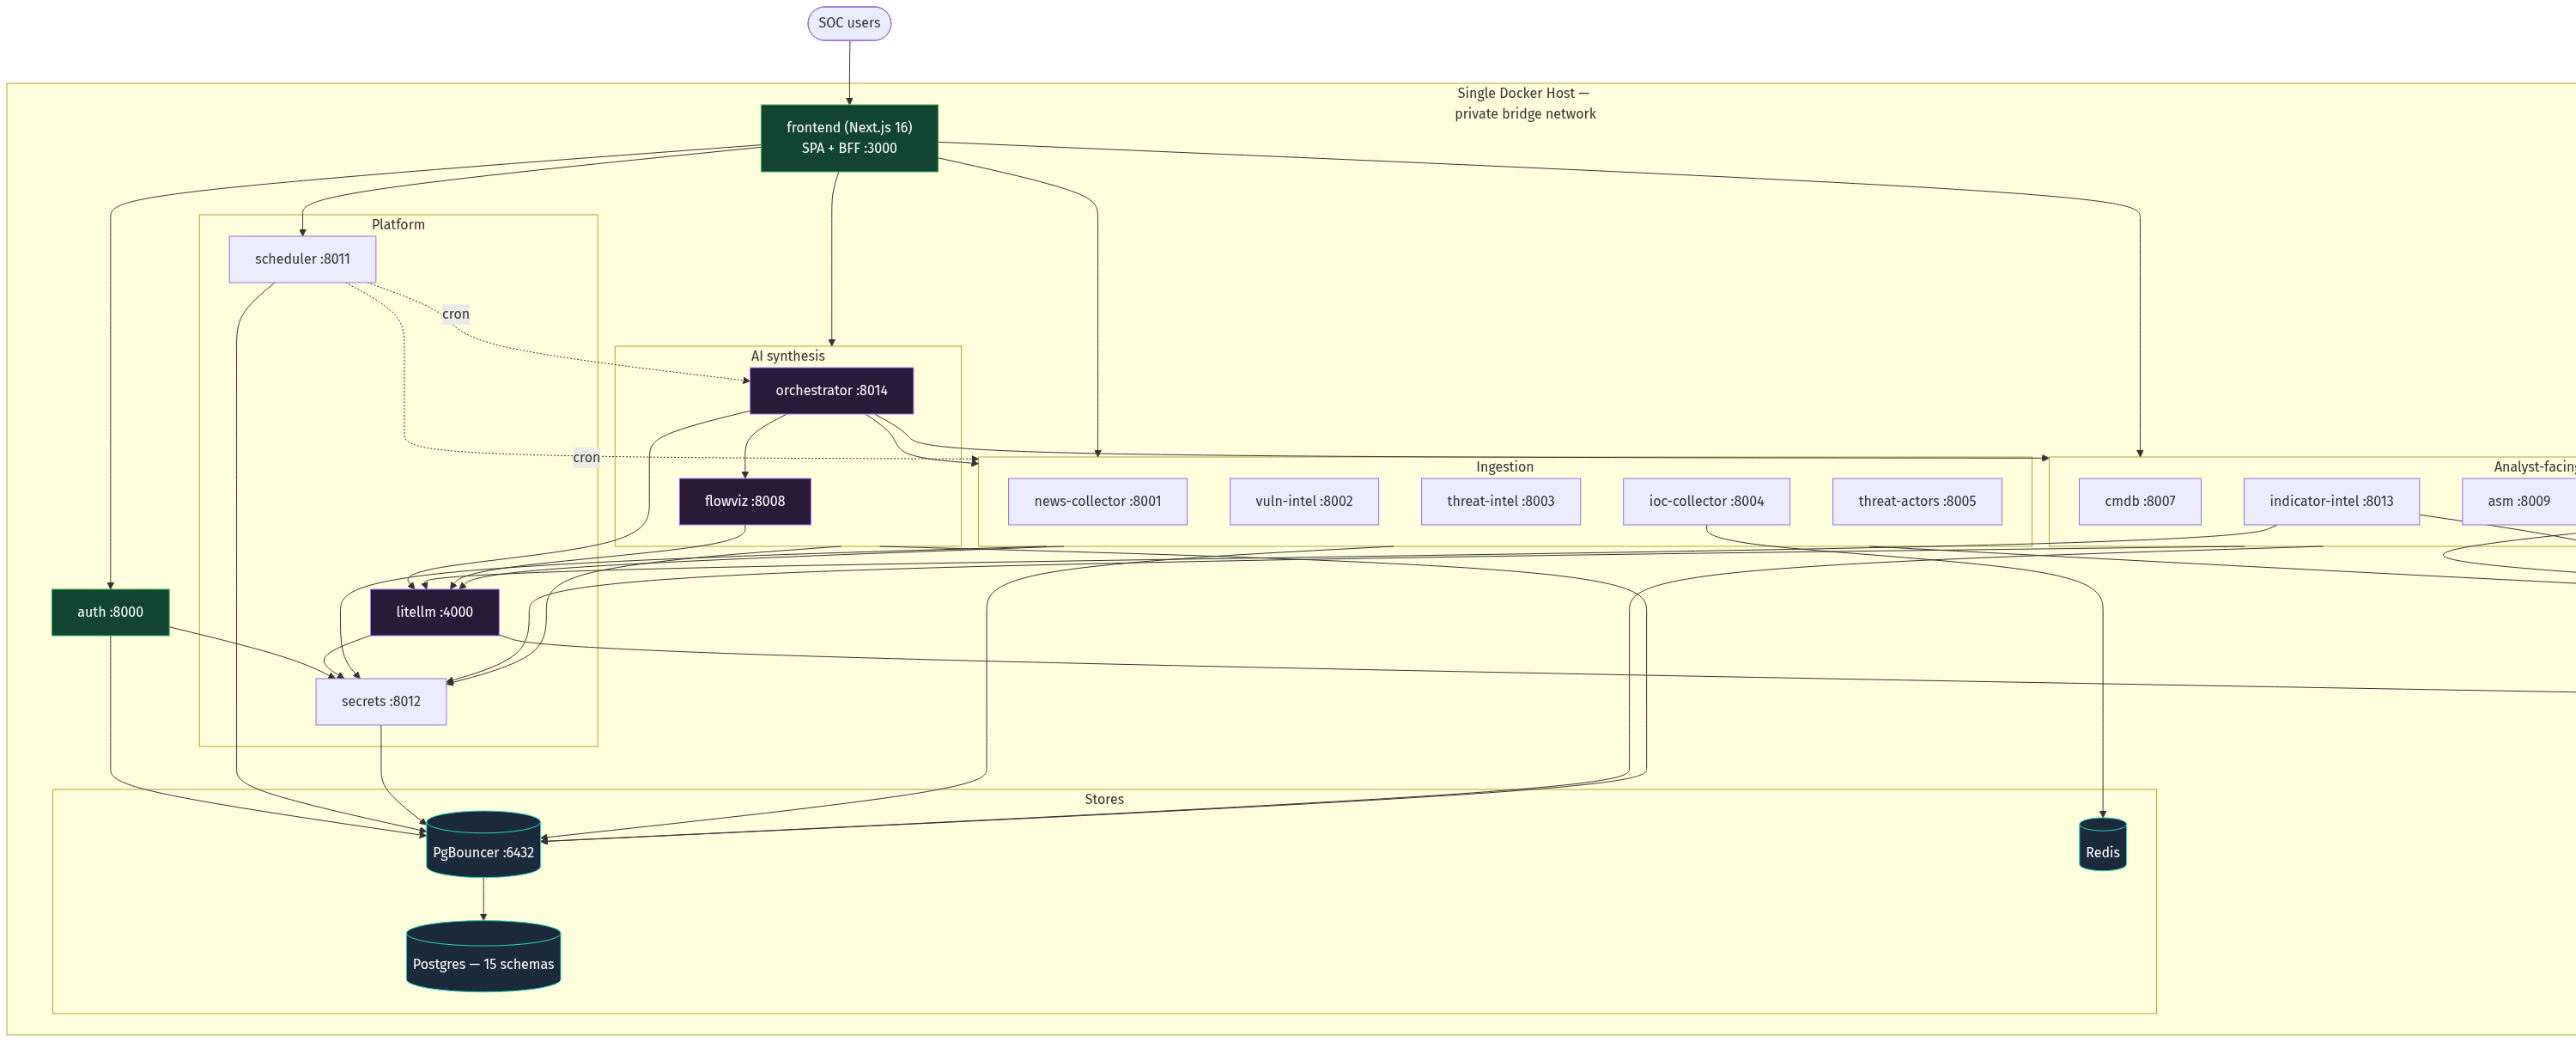
\includegraphics[width=\textwidth]{images/tip/diagrams/05_global_architecture_core.png}
\caption{Global system architecture, core platform topology.}
\label{fig:global-arch}
\end{figure}

\begin{figure}[H]
\centering
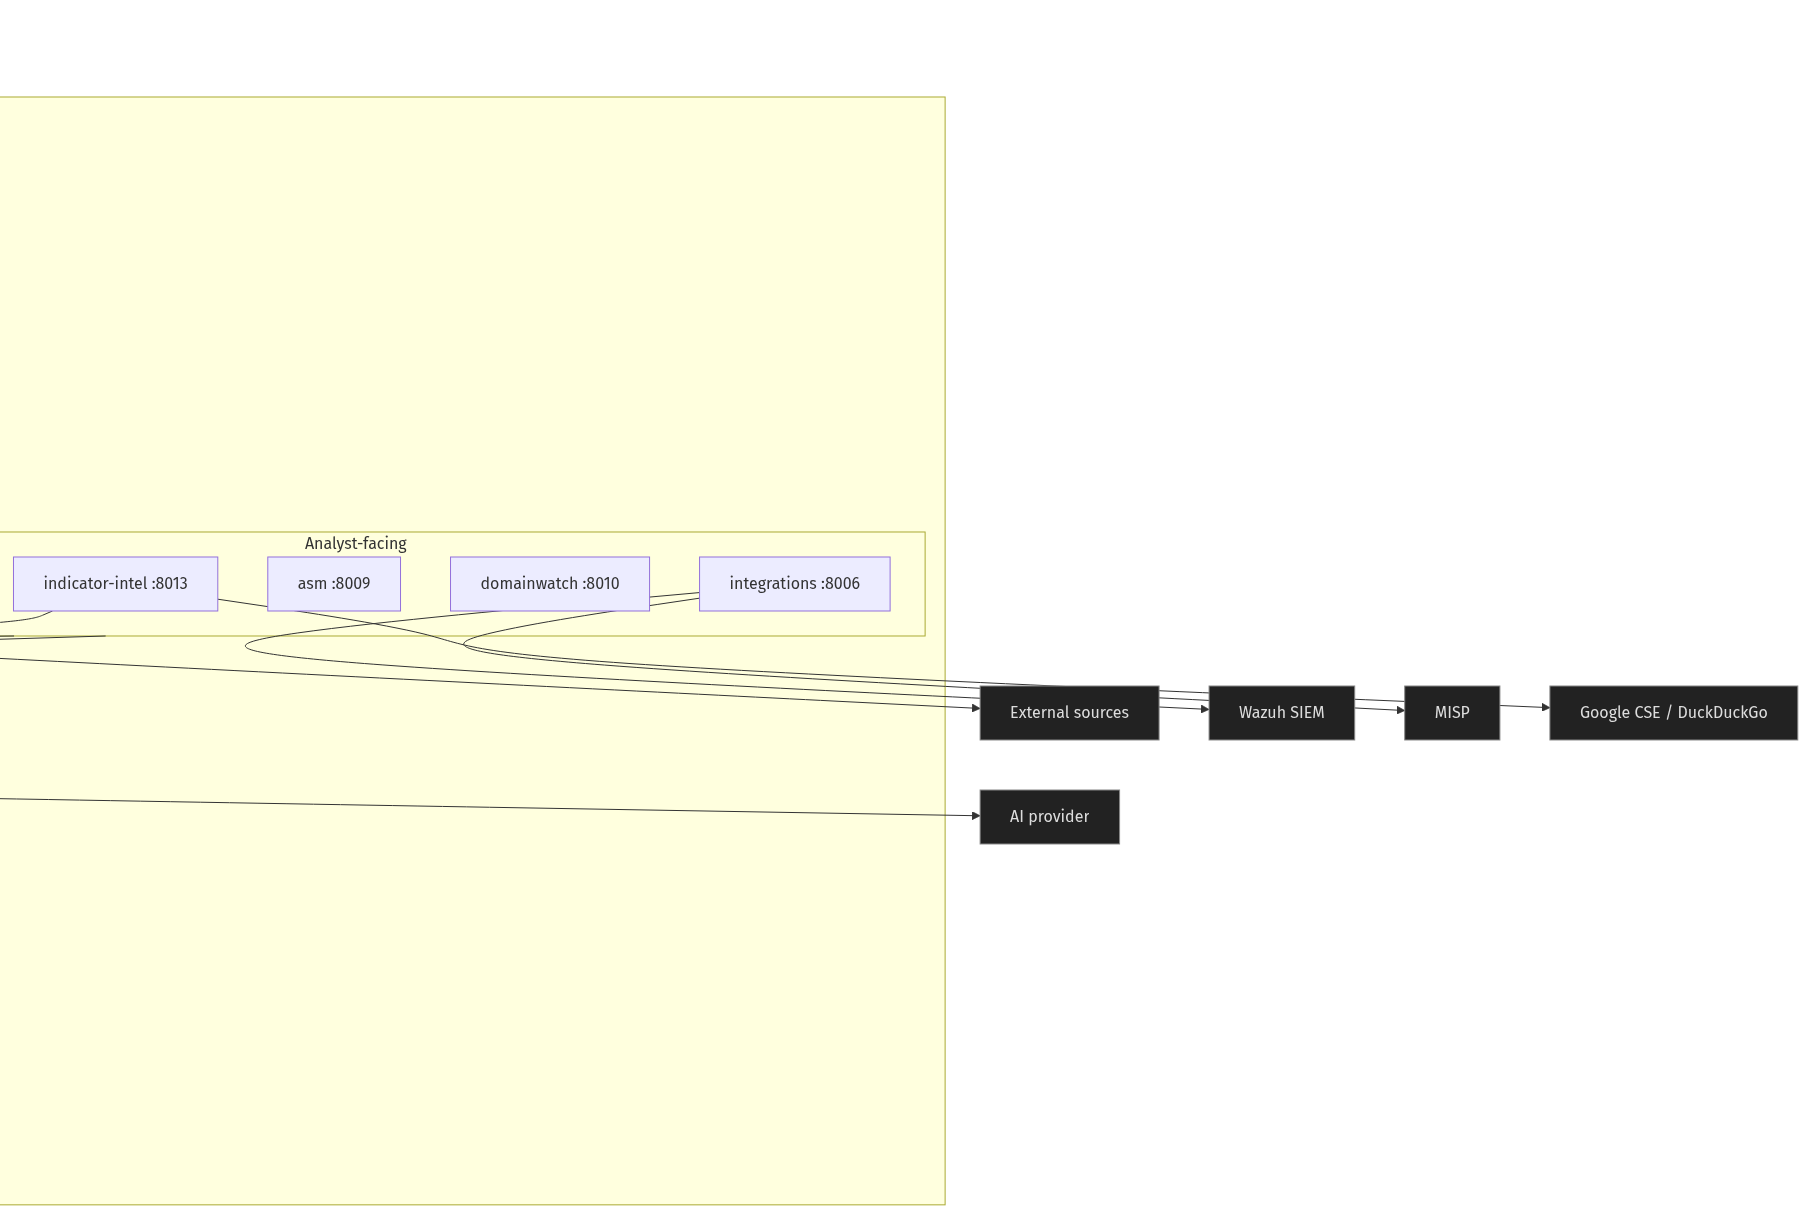
\includegraphics[width=0.92\textwidth]{images/tip/diagrams/05_global_architecture_integrations.png}
\caption{Global system architecture, analyst-facing edge and external integrations.}
\label{fig:global-arch-ext}
\end{figure}

\begin{table}[H]
\centering
\caption{Service catalogue and primary responsibility}
\label{tab:service-catalogue-new}
\renewcommand{\arraystretch}{1.2}
\begin{tabular}{|p{3.2cm}|p{2.2cm}|p{1.5cm}|p{6.0cm}|}
\hline
\textbf{Service} & \textbf{Layer} & \textbf{Port} & \textbf{Primary responsibility}\\
\hline
auth & platform & 8000 & user login, refresh tokens, RBAC, service identity\\
\hline
news-collector & ingestion & 8001 & article feed ingestion and article views\\
\hline
vuln-intel & ingestion & 8002 & CVE, EPSS, KEV refresh and vulnerability views\\
\hline
threat-intel & ingestion & 8003 & public threat reporting, supply-chain and breach context\\
\hline
ioc-collector & ingestion & 8004 & indicator ingestion, normalization, lookup\\
\hline
threat-actors & ingestion & 8005 & actor, ransomware, TTP and tool intelligence\\
\hline
integrations & analyst & 8006 & Wazuh and MISP integration surfaces\\
\hline
cmdb & analyst & 8007 & assets, tags, company profile, organizational context\\
\hline
flowviz & synthesis & 8008 & attack-flow generation and rendering support\\
\hline
asm & analyst & 8009 & passive attack-surface discovery workflows\\
\hline
domainwatch & analyst & 8010 & domain monitoring and screenshot capture\\
\hline
scheduler & platform & 8011 & recurring jobs and run-history management\\
\hline
secrets & platform & 8012 & encrypted secret storage and bootstrap fetch\\
\hline
indicator-intel & analyst & 8013 & deep indicator investigation and dorking workflows\\
\hline
orchestrator & synthesis & 8014 & AI synthesis, reporting, Q\&A, policies, actions\\
\hline
\end{tabular}
\end{table}

\section{Architectural Decomposition}
\subsection{Ingestion Services}
The ingestion layer is responsible for obtaining intelligence from external providers, transforming it into a stable internal shape, and storing it durably. Each service owns one intelligence domain, which limits failure blast radius and keeps external-source logic localized. News, vulnerabilities, indicators, actors, and threat reporting are therefore refreshed independently and can degrade independently.

\subsection{Analyst-Facing Services}
The analyst layer exposes the context required to interpret intelligence operationally. CMDB represents assets and the organization profile. Integrations exposes operational telemetry from Wazuh and MISP. ASM and domainwatch provide exposure-oriented views that complement pure threat feeds. Indicator-intel performs slower, investigation-grade enrichment when a quick IOC verdict is insufficient.

\subsection{Synthesis Services}
The synthesis layer is centred on the orchestrator. It does not ingest raw feeds directly. Instead, it fans out over the other services' HTTP interfaces, assembles context, executes structured AI analysis, and persists outputs such as reports, rankings, and correlations. Flowviz complements this by generating graphable attack-flow structures from textual or analytical inputs.

\subsection{Platform Services}
The platform layer contains the shared control-plane functions: authentication, secret management, scheduling, and AI gatewaying. Centralizing these concerns reduces duplication and keeps high-sensitivity logic in a small number of services.

This four-layer decomposition also reflects a theoretical distinction between data acquisition, context exposure, analytical transformation, and platform governance. The ingestion layer acquires and shapes knowledge. The analyst layer exposes organization-specific context and operational surfaces. The synthesis layer performs cross-domain reasoning. The platform layer governs trust, configuration, and execution. This separation is useful academically because it explains why similarly technical components belong to different layers: the criterion is not implementation language or container image, but role in the knowledge-production process.

\section{Backend Architecture and Shared Service Shape}
All backend services share one construction pattern. The shared factory in \texttt{tip\_common} configures structured logging, correlation-ID middleware, error handlers, and a health endpoint. Startup hooks then initialize per-service state such as database engines, cache clients, secret clients, source-health repositories, AI clients, and scheduler instances. Auth middleware is intentionally not added in the shared factory because services often need to fetch the verification key during startup before requests can be validated.

This pattern is important architecturally because it delivers two forms of consistency at once. Services remain thin and domain-focused, but operational concerns such as logging, correlation, error translation, and settings handling are solved once in the shared layer. Figure~\ref{fig:module-deps} shows the dependency direction between services and shared libraries.

From a software-engineering perspective, this is a deliberate use of an internal platform layer. Instead of expecting each service to rediscover how to log, manage settings, expose health, handle correlation IDs, or map exceptions, the shared packages encode those concerns once and make them cheap to reuse. The result is a service portfolio with lower accidental variation. This matters because in multi-service systems, ungoverned local variation often becomes a larger source of operational fragility than the domain logic itself.

\begin{figure}[H]
\centering
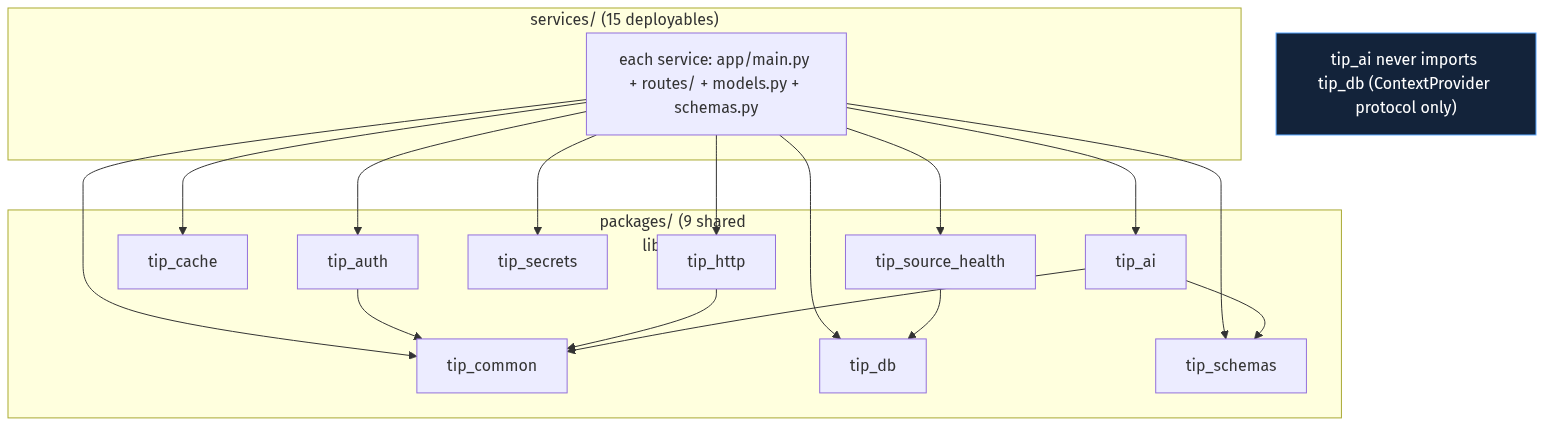
\includegraphics[width=0.92\textwidth]{images/tip/diagrams/14_module_dependencies.png}
\caption{Dependency direction between shared packages and services.}
\label{fig:module-deps}
\end{figure}

\section{Frontend Architecture and the BFF Pattern}
The frontend is a Next.js application using the App Router. Its role is more significant than a simple presentation layer. It serves as the browser-facing entry point and hosts the backend-for-frontend proxy under \texttt{/api/*}. The catch-all BFF route maps path prefixes to backend services and forwards headers, query parameters, and request bodies accordingly.

This design provides three concrete benefits. First, it gives the browser one consistent origin and one consistent API surface. Second, it keeps backend service URLs and routing logic centralized in one place. Third, it allows the frontend to expose aggregate routes such as the dashboard endpoint, which fans out to multiple services in parallel and returns a single response tailored to the user interface.

The frontend stores user state and permissions in a persisted client-side store and uses that state to attach Bearer tokens to BFF requests. This must be stated precisely because it differs from a stricter cookie-only edge model. The current deployment relies on client-held tokens plus a BFF proxy, not on HTTP-only cookie injection.

Theoretically, the BFF layer resolves a representational mismatch. Backend services are designed around domain ownership, not around page composition. A dashboard, for example, is not a natural object in the vulnerability or actor services by themselves. It is a frontend concern that requires aggregated, latency-aware composition. The BFF therefore improves not only security posture but also interface ergonomics. It allows the user interface to evolve without forcing every backend service to become UI-aware.

\section{Request and Communication Patterns}
The platform is deliberately message-light. The dominant coordination mechanism is HTTP, both from browser to BFF and between internal services. Figure~\ref{fig:req-flow} illustrates the main request lifecycle.

\begin{figure}[H]
\centering
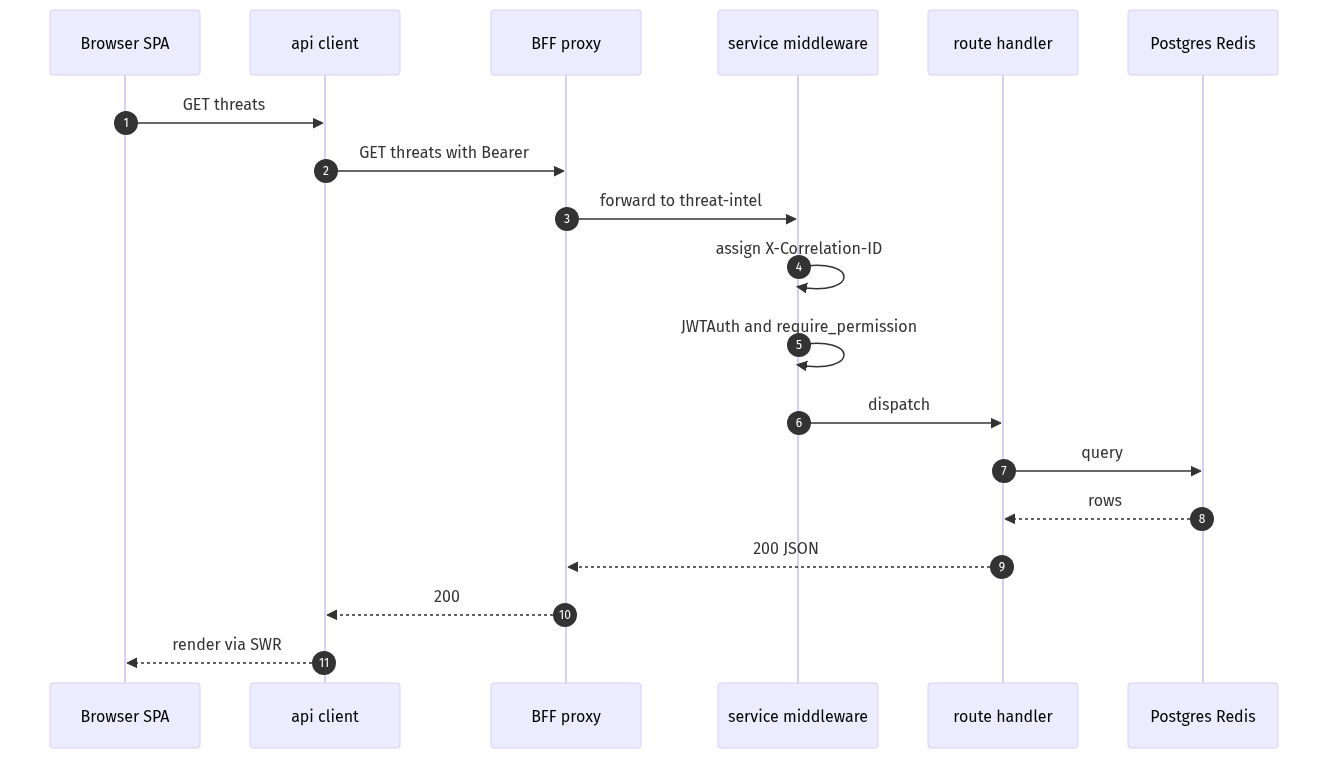
\includegraphics[width=0.92\textwidth]{images/tip/diagrams/05_request_flow.png}
\caption{Request flow from frontend to backend services.}
\label{fig:req-flow}
\end{figure}

Four recurring communication patterns appear across the system.

\subsection{Synchronous Read Paths}
Most read endpoints return stored data directly from Postgres, optionally mediated by Redis for hot lookups. This keeps user-visible latency bounded by local infrastructure rather than external feeds.

\subsection{Scheduler-Triggered Control Paths}
Recurring work is initiated by the scheduler through HTTP POST calls that carry a generated run identifier. Endpoints may complete synchronously or accept work and complete it asynchronously via callback. This pattern preserves a simple control plane while still supporting long-running jobs.

\subsection{Context Fan-Out}
The orchestrator performs multi-leg fan-out calls to assemble the context needed for synthesis. It does not bypass service boundaries by reading their tables directly. This is one of the strongest indicators that the service decomposition is real rather than nominal.

\subsection{Bootstrap and Secret Retrieval}
Services use a pre-authentication bootstrap path to obtain secrets needed before they have a JWT. The same pattern is used to obtain the auth public key and service bootstrap tokens during startup.

Figure~\ref{fig:service-interactions} summarizes the most important inter-service interactions.

\begin{figure}[H]
\centering
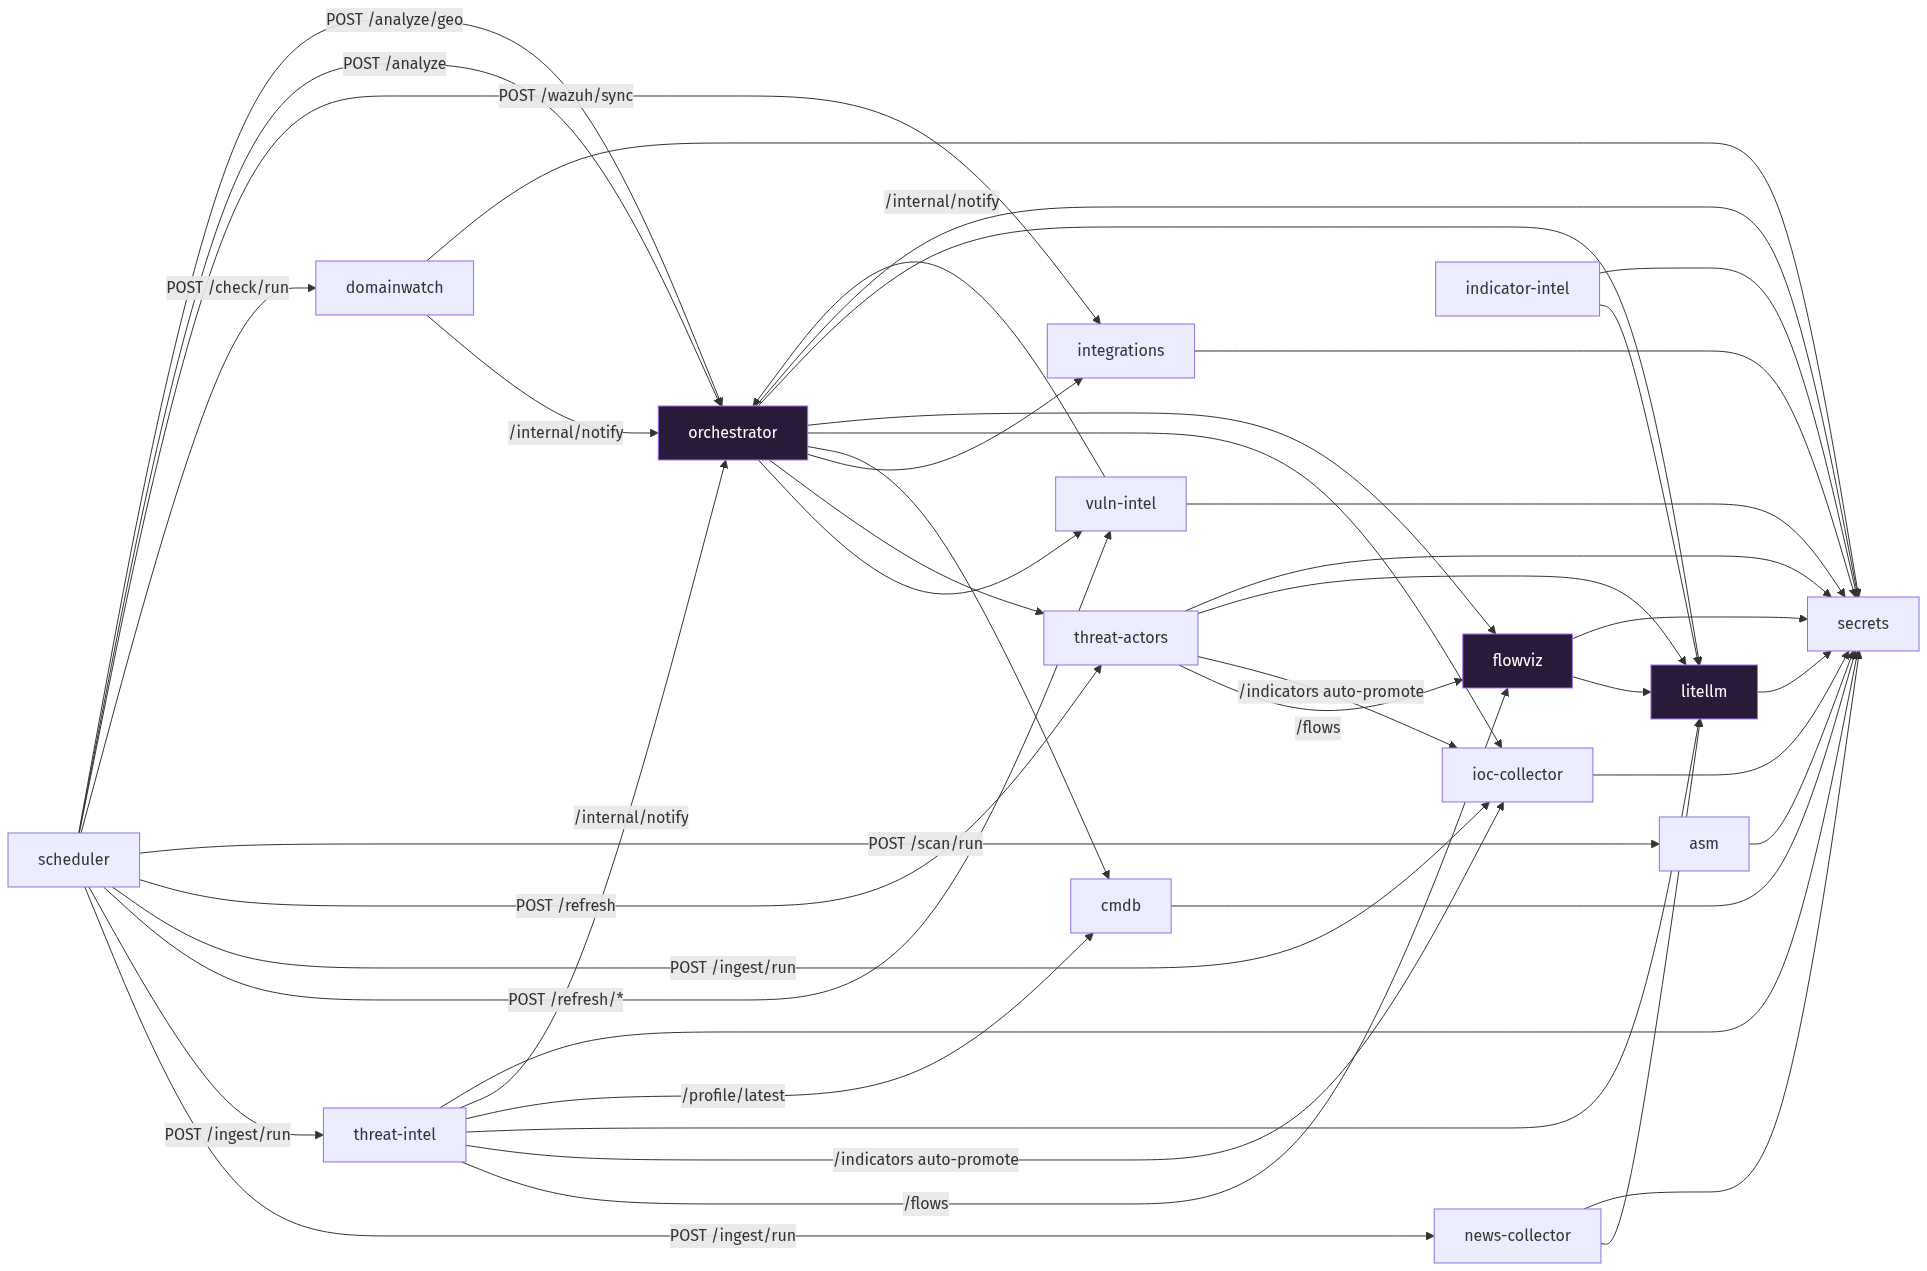
\includegraphics[width=0.95\textwidth]{images/tip/diagrams/05_service_interactions.png}
\caption{Primary inter-service interactions.}
\label{fig:service-interactions}
\end{figure}

\section{Data Architecture}
\subsection{One Database, Many Schemas}
All services share one PostgreSQL database, but logical isolation is maintained by schema partitioning. Each service owns its own schema, migrations, and ORM models. No foreign key crosses a schema boundary. Cross-service relations are resolved through stable identifiers and HTTP APIs rather than joins across tables.

This design is a compromise between operational simplicity and service isolation. A database-per-service model would have increased operational cost significantly for the target deployment. A single shared schema would have undermined modularity. The chosen approach preserves one backup domain and one database process while still allowing per-service ownership.

The database architecture is therefore best understood as a layered compromise. It accepts a shared physical store while preserving logical ownership boundaries. This avoids a common false binary in service-oriented design: either every service gets its own full infrastructure stack, or all services collapse into one undifferentiated data model. The chosen solution preserves the migration path toward stronger physical separation later without paying the operational cost upfront.

\begin{figure}[H]
\centering
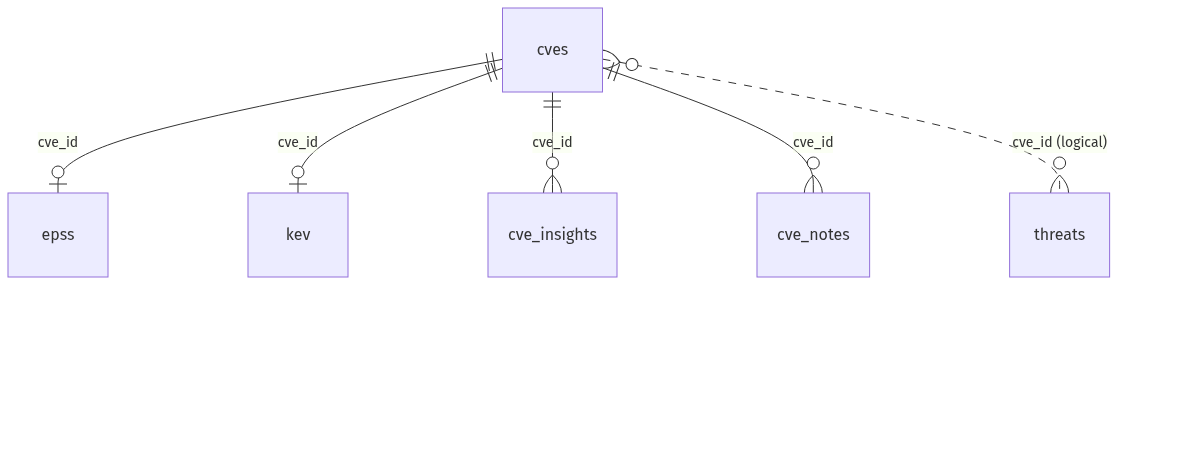
\includegraphics[width=\textwidth]{images/tip/diagrams/07_erd_left.png}
\caption{High-level entity relationship structure across service schemas, part 1.}
\label{fig:erd-new}
\end{figure}

\begin{figure}[H]
\centering
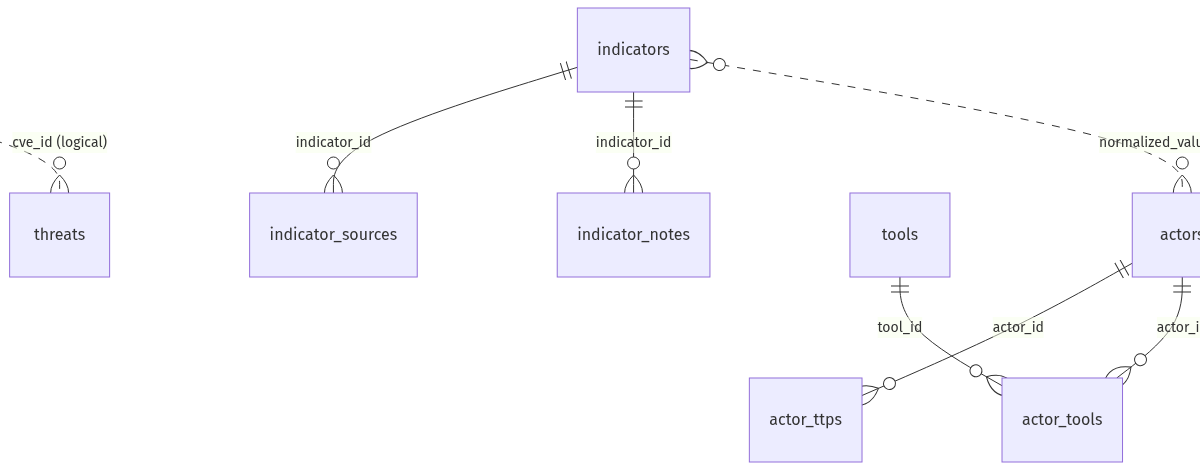
\includegraphics[width=\textwidth]{images/tip/diagrams/07_erd_center.png}
\caption{High-level entity relationship structure across service schemas, part 2.}
\end{figure}

\begin{figure}[H]
\centering
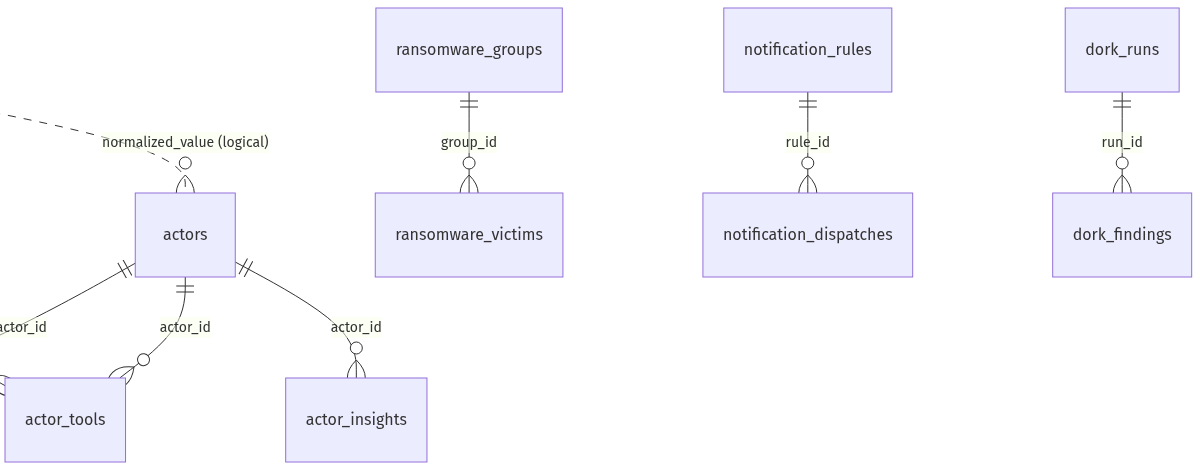
\includegraphics[width=\textwidth]{images/tip/diagrams/07_erd_right.png}
\caption{High-level entity relationship structure across service schemas, part 3.}
\end{figure}

\subsection{PgBouncer and Pooler-Aware Access}
PgBouncer sits between application services and Postgres in transaction-pooling mode. This is not a cosmetic optimisation. It allows fifteen services to share a bounded set of backend connections without exhausting the database. It also imposes constraints on the SQLAlchemy configuration: prepared-statement caching is disabled and connections are pre-pinged and recycled to tolerate pooler behaviour and stale backends.

\begin{figure}[H]
\centering
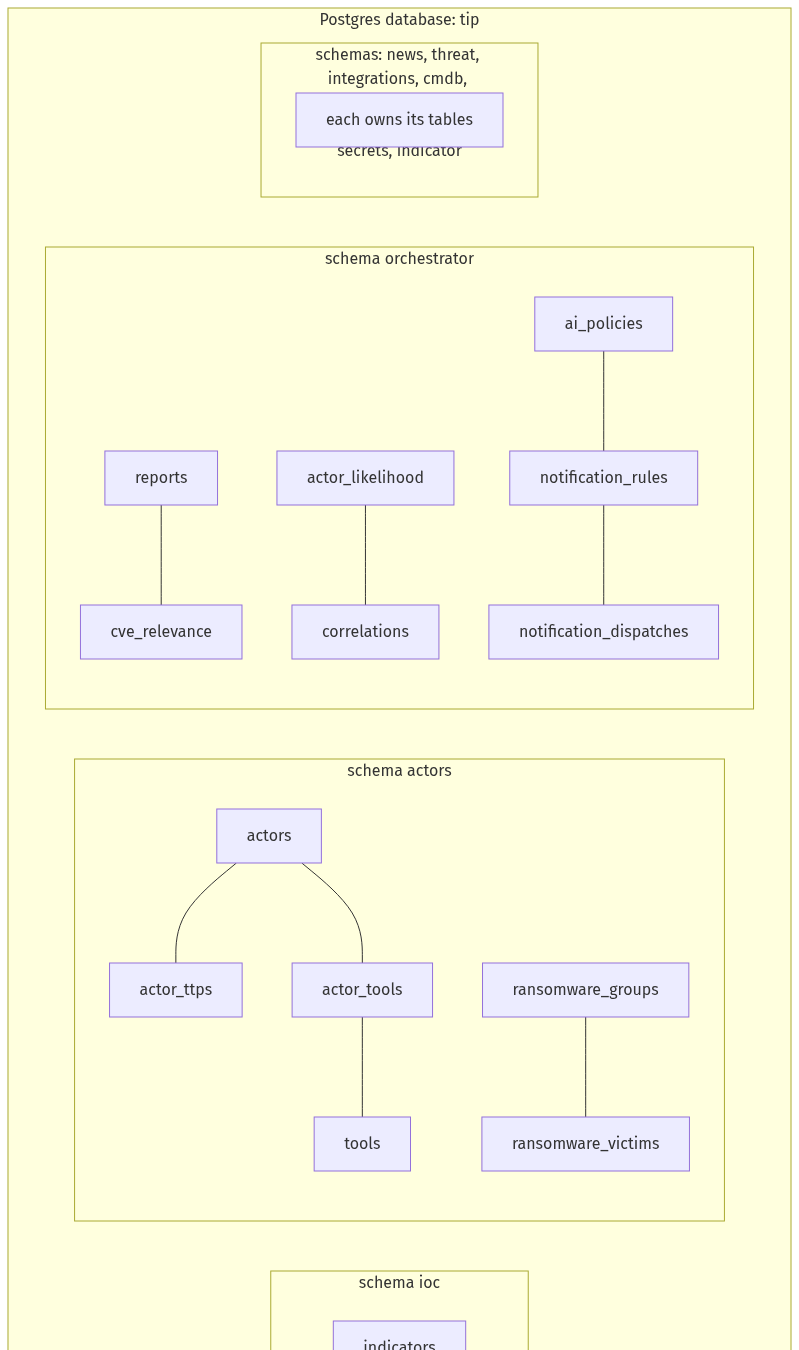
\includegraphics[width=0.74\textwidth]{images/tip/diagrams/07_relational_model_top.png}
\caption{Relational topology with PgBouncer between services and PostgreSQL, upper segment.}
\label{fig:relational-model-new}
\end{figure}

\begin{figure}[H]
\centering
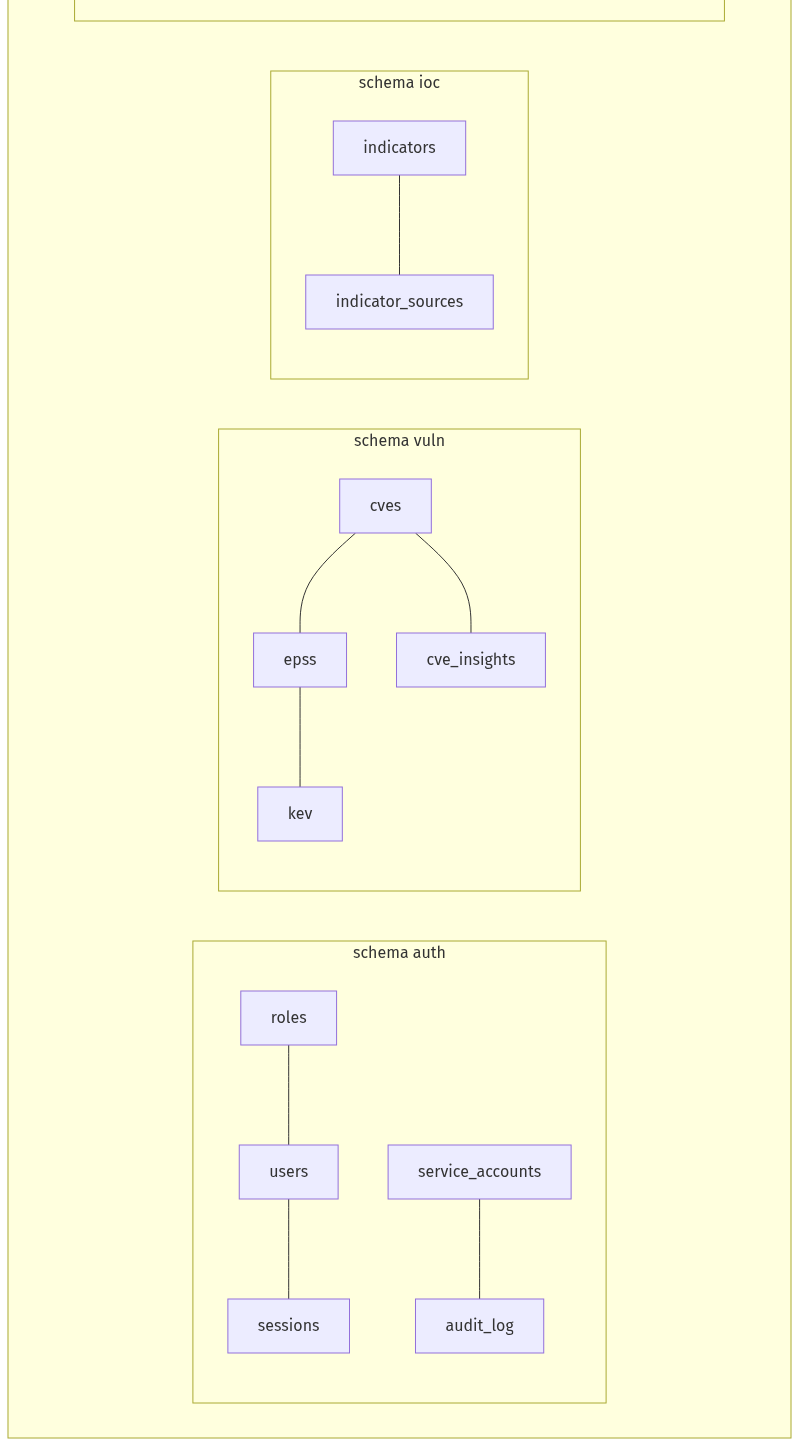
\includegraphics[width=0.74\textwidth]{images/tip/diagrams/07_relational_model_bottom.png}
\caption{Relational topology with PgBouncer between services and PostgreSQL, lower segment.}
\end{figure}

\subsection{JSON for Fidelity, Relational Columns for Queries}
Many records retain upstream payloads in JSON form while also extracting searchable relational fields. This is an important engineering choice. The relational columns support fast query patterns, sorting, and filtering. The JSON payloads preserve source fidelity and support reprocessing without having to fetch historical data again.

This hybrid storage model addresses a common tension in intelligence systems. Purely relational schemas are excellent for structured query and constraint enforcement, but they can be too rigid for heterogeneous and evolving source payloads. Pure document storage preserves source richness but can make common analytical queries and joins inefficient or ambiguous. By combining relational projections with retained upstream JSON, the platform preserves both operational queryability and evidentiary fidelity.

\section{Authentication, Authorization, and Trust Boundaries}
\subsection{Actual Trust Model}
The trust model must be described carefully. The auth service validates user credentials, issues RS256 access tokens and refresh tokens, and exposes role and session administration. However, in the current Docker Compose deployment, most non-auth services inherit \texttt{DISABLE\_AUTH=true} on the private Docker network, while auth itself runs with enforcement enabled. In practice, this means the platform's strongest trust boundary is between the browser-facing layer and the internal service network, not between every pair of internal services.

This is a deliberate simplification, not an implementation accident. It reduces failure modes associated with service-to-service token validation, but it also weakens internal segmentation. Any academic treatment of the platform must present both sides of that tradeoff.

\subsection{RBAC Enforcement}
Where auth is enforced, permissions are checked through a single shared dependency, \texttt{require\_permission}. This keeps authorization logic declarative at route level and makes permission intent visible in code. The auth service's \texttt{/me} route rehydrates the current user state from the database instead of trusting stale JWT claims, which is a stronger pattern than naive claim-only identity handling.

\subsection{Secrets Management}
All secrets except the Fernet key and the shared bootstrap token are stored in the secrets service, encrypted at rest. Services fetch required secrets during startup. Access to secrets is audited. The LiteLLM proxy retrieves provider API keys from the vault at startup, which means downstream analytical services generally hold only the proxy master key rather than direct provider credentials.

From a design-theory perspective, the trust model is intentionally asymmetric. User-originated traffic is handled with much stronger authentication expectations than internal service-to-service traffic in the current deployment profile. This is not the purest possible design, but it is legible and defensible if described honestly. It reduces some operational coupling while preserving a clear future hardening path toward stronger internal verification.

\section{Security Boundary and External Exposure}
The deployment aims to minimize external exposure, but the reality must be stated accurately. The frontend is the intended browser-facing application. However, the compose file also publishes several backend ports for direct access and diagnostics. The architecture should therefore be described as a deployment with a primary edge at the frontend plus additional exposed service ports, not as a perfectly single-port system.

This distinction matters because it affects how the security chapter should reason about hardening, monitoring, and future improvements.

\section{Caching and Source Health as Architectural Components}
Redis is used as a loss-tolerant accelerator rather than as a system of record. Hot-path indicator results, transient AI responses, and source-health state are cached with bounded TTLs. The durable source of truth remains PostgreSQL. The source-health subsystem spans cache and database: Redis provides fast checks for open circuits, while the per-service source-health tables provide durable operator visibility.

This is architecturally important because cache and health state are not treated as incidental implementation details. They are part of the system's control logic. Source health influences whether the platform should continue attempting upstream calls. Cache state influences whether the platform can respond at operational speed. In that sense, both are first-class architectural elements rather than mere optimizations.

\section*{Conclusion}
\addcontentsline{toc}{section}{Conclusion}
The delivered architecture is a modular, HTTP-coordinated, single-host security platform shaped more by operational clarity than by distributed-systems maximalism. Its strongest properties are consistent service construction, clear domain boundaries, schema ownership, explicit control-plane services, and a practical BFF layer. Its most important caveat is that the internal trust model is simpler and more permissive than a strict service-mesh security story would suggest. The next chapter explains the platform technologies and infrastructure stack that make this architecture operationally viable, before the report turns to the service catalogue and implementation mechanics.
